\subsection{Vector Display}
A vector display/monitor, is a screen device that displays graphics by drawing from point to point. 
This is different than a raster display, which is described in the next section.
All vector monitors utilize CRT (Cathode Ray Tube) technology, which contain one or more electron emitters that fire electron beams that are deflected onto a phosphorescent screen to display images.

Unlike the CRT raster displays in old television sets or computer monitors, a vector monitor does not scan repeatedly in a fixed pattern. 
It instead draws lines by gradually firing the electron beam to a point defined by two voltages, one defining the horizontal placement X and one defining the vertical Y. 
Once a line is drawn, the electron emitter stops firing and moves to the starting point of the next line, thus leaving out dark areas. 
This process is shown in figure \ref{fig:vectorscan}.

\begin{figure}[h!]
\centering 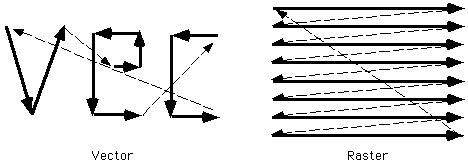
\includegraphics[width=0.8\linewidth]{images/scan.png}
\caption{Scan comparison between vector graphics (left) and raster graphics (right). Source: \cite{vecvsras}}
\label{fig:vectorscan}
\end{figure}

Refresh rate depends on which type of phosphor is used. 
Some phosphor types fade out very quickly and needs refreshing 30-40 times per second.
Special types of phosphor can last for several minutes.

The basic vector display is monochromatic. 
However, certain displays with color support exist. 
By using a shadow mask - that is a perforated plate that acts as a filter - between the electron guns and the screen, and having one electron gun for red, green and blue, RGB colors can be displayed on the screen.

Notable advantages with vector displays are:
\begin{itemize}
\item Since they are able to draw directly from one point to another, they do not suffer from artifacts such as aliasing and pixelation.
\item The entire screen is not updated every time, only the areas that the electron beam visits.
\end{itemize}

There are, however, some major disadvantages:
\begin{itemize}
\item Graphic detail on vector displays are very limited compared to raster screens, because of crude line drawings and often limited color support.
\item The refresh rate is also limited. When a bigger area of the screen is drawn, the screen starts to flicker more and more.
\item Irregular electron beam motion is slower than raster screens' predictable scanning.
\end{itemize} 

Vector displays are pretty much obsolete today, because of raster screens' inexpensiveness and support for graphics with a higher level of detail. 
Algorithms for graphics generation on raster screens are also much simpler than corresponding algorithms for vector screens.

\subsubsection{Oscilloscope}
An oscilloscope is a popular lab tool used to output voltage as a function of time.
Modern oscilloscopes often use thin film transistor (TFT) displays and rasterize output. 
However, older models include a CRT display, and can thus act as a vector display.

To draw on such an oscilloscope, the device must support at least two input channels, and the ability to draw in X-Y mode.
This means that two of the input channels (usually Ch1 and Ch2) governs the electron ray deflectors, which are controlled through electrostatics.
If the channels are provided with a constant voltage, a dot will be displayed on the screen - in contrast to normal mode, where a line would be drawn. // TODO: What is 'normal' mode? Varying voltage?

The voltage on channel one will normally decide the beam's horizontal X position, and channel two its vertical Y position.
To draw a line on the oscilloscope, one would need to repeatedly change the voltage of one or both channels back and forth. // TODO: Why does this happen?
Changing the voltage on only one channel will produce a horizontal or vertical line. // TODO: Why does this happen?
